\documentclass[10pt]{article}
\usepackage[margin=1in,headsep=14pt,headheight=15pt]{geometry}
\usepackage{amsmath,amsthm}\usepackage{unicode-math}
\setmainfont{OldStandard}[Path=fonts/,Extension=.otf,UprightFont=*-Regular,ItalicFont=*-Italic,BoldFont=*-Bold,BoldItalicFont=*-BoldItalic,Ligatures=TeX,Numbers=Lining]
\setmathfont{OldStandard-Math.otf}[Path=fonts/,Scale=MatchLowercase]
\setmathfont{OldStandard-Regular.otf}[Path=fonts/,range={up/num}]
\setmathrm{OldStandard}[Path=fonts/,Extension=.otf,UprightFont=*-Regular,ItalicFont=*-Italic,BoldFont=*-Bold,BoldItalicFont=*-BoldItalic]
\makeatletter\renewcommand\normalsize{\@setfontsize\normalsize{10.5pt}{12.9pt}\abovedisplayskip 8pt plus2pt minus4pt\abovedisplayshortskip 0pt plus2pt\belowdisplayshortskip 4pt plus2pt minus2pt\belowdisplayskip\abovedisplayskip}\makeatother\normalsize
\usepackage{placeins}\usepackage{needspace}
\usepackage{microtype,booktabs,graphicx,enumitem,tabularx,multirow}
\newsavebox{\manuscripttable}
\newenvironment{fittable}{\begin{lrbox}{\manuscripttable}}{%
\end{lrbox}\ifdim\wd\manuscripttable>\linewidth
\resizebox{\linewidth}{!}{\usebox{\manuscripttable}}%
\else\usebox{\manuscripttable}\fi}
\usepackage[table]{xcolor}
\definecolor{accent}{HTML}{262626}
\definecolor{rule}{HTML}{D4D4D4}
\usepackage[numbers,sort&compress]{natbib}
\usepackage[skins]{tcolorbox}
\usepackage[colorlinks,linkcolor=accent,citecolor=accent,urlcolor=accent]{hyperref}
\usepackage{caption}
\captionsetup{font=small,labelfont={bf,color=accent},labelsep=period,margin=0pt}
\usepackage{titlesec}
\titleformat{\section}{\large\bfseries\color{accent}}{\thesection}{0.7em}{}
\titleformat{\subsection}{\normalsize\bfseries\color{accent}}{\thesubsection}{0.6em}{}
\titlespacing*{\section}{0pt}{1.6ex plus .5ex}{1.0ex}
\titlespacing*{\subsection}{0pt}{1.3ex plus .4ex}{0.6ex}
\titlespacing*{\paragraph}{0pt}{1.4ex plus .4ex minus .2ex}{0.8em}
\titleformat{\paragraph}[runin]{\normalsize\bfseries\color{accent}}{}{}{}
\usepackage{fancyhdr}
\pagestyle{fancy}\fancyhf{}
\fancyhead[L]{\small\color{gray}{\addfontfeature{LetterSpace=5}\textsc{Mad in Herds}}}
\fancyhead[R]{\small\color{gray}{\addfontfeature{LetterSpace=5}\textsc{Apart Research}}}
\fancyfoot[C]{\footnotesize\thepage}
\renewcommand{\headrulewidth}{0.4pt}\renewcommand{\headrule}{\vspace{3pt}{\color{rule}\hrule width\headwidth height\headrulewidth}}
\setlist{nosep,leftmargin=1.3em}
\emergencystretch=3em\hfuzz=1.5pt
\newtheoremstyle{manuscript}{9pt}{6pt}{\normalfont}{}{\bfseries}{.}{0.6em}{}
\theoremstyle{manuscript}\newtheorem{proposition}{Proposition}
\newcommand{\E}{\mathbb E}
\newcommand{\Var}{\operatorname{Var}}
\newcommand{\Cov}{\operatorname{Cov}}
\hypersetup{pdftitle={Mad in Herds: AI Assistants Amplify a Biased Crowd},pdfauthor={Vikram Viswanath},bookmarksnumbered=true}
\renewenvironment{abstract}{\begin{center}{\addfontfeature{LetterSpace=12}\textsc{abstract}}\end{center}\vspace{-0.5em}\list{}{\leftmargin=0.5in\rightmargin=0.5in\listparindent=0pt\itemindent=0pt}\item\relax\linespread{1.08}\selectfont}{\endlist}
\newcommand{\Dw}{D_{\mathrm{within}}}
\newcommand{\Db}{D_{\mathrm{between}}}
\newcommand{\Dx}{D_{\mathrm{excess}}}
\newcommand{\pH}{p_{\text{Holm}}}
\definecolor{good}{HTML}{15803D}\definecolor{mid}{HTML}{B45309}\definecolor{weak}{HTML}{C2410C}
\newcommand{\strongc}{\textcolor{good}{\textbf{Strong}}}
\newcommand{\moderate}{\textcolor{mid}{\textbf{Moderate}}}
\newcommand{\weakc}{\textcolor{weak}{\textbf{Not shown}}}

\newcommand{\suggest}{\textcolor{mid}{\textbf{Suggestive}}}
\newcommand{\inconc}{\textcolor{mid}{\textbf{Inconclusive}}}
\newcommand{\notsup}{\textcolor{weak}{\textbf{Not supported}}}

\title{\vspace{-4.2em}{\color{accent}\rule{\linewidth}{1.2pt}}\\[10pt]
{\LARGE\bfseries\color{accent} Mad in Herds: AI Assistants\\[2pt] Amplify a Biased Crowd}\\[8pt]
{\large\itshape Biased consensus amplifies error. A short critique partially offsets the harm.}\\[4pt]
{\color{accent}\rule{\linewidth}{0.5pt}}}
\author{\large Vikram Viswanath\\[1pt] \normalsize University of Sydney\\[3pt] \normalsize With Apart Research\thanks{Research conducted at the AI$\times$Epistemics Research Sprint (November 2026).}}
\date{\vspace{-2.2em}}

\begin{document}
\maketitle\thispagestyle{plain}

\begin{abstract}
\noindent Can a consensus signal make AI advice less accurate? Eight simulated agents sharing a misconception each consult an LLM assistant about quantities with known answers. In a discovery study (16 tasks) and a replication under a committed analysis plan (40 new tasks, three replicates), showing the assistant the crowd's median and interquartile range increased final crowd error relative to the same model without peer statistics. Final crowd error more than doubled with \mbox{Gemma-4-26B} ($+115\%$, worse on 36 of 40 tasks) and rose with DeepSeek ($+106\%$), Qwen ($+29\%$), GLM ($+24\%$) and a four-model panel ($+64\%$; all $\pH\le0.003$), though the assistants still improved on the crowd's starting point. An exact accounting identity places 56--69\% of the added error in the product of the crowd's and assistants' signed errors. A 53-word critique of both the user's estimate and the crowd consensus beat length-matched generic reflection ($\pH=0.0005$) but recovered only about half of Gemma's added error; the discovery study's near-full recovery did not replicate. Finally, an elementary variance identity shows why pooled single-model baselines conflate static averaging with interaction. Against a seat-matched virtual panel that preserves the aggregation rule, mixing reduced error modestly ($-8\%$).
\end{abstract}

\begin{list}{}{\leftmargin=0.5in\rightmargin=0.5in\topsep=4pt}\item\relax
{\small\textbf{Epistemic status.} The harm replicates in all four model families under a plan committed before data collection, but is measured against silent assistants, not the crowd's starting point. The critique's benefit is partial; The discovery estimate did not replicate. The decomposition is accounting, not causal. Agents are simulated. Appendix~\ref{sec:cruxes} grades every claim.\par}
\end{list}

\vfill
\noindent\begin{minipage}{\linewidth}\centering
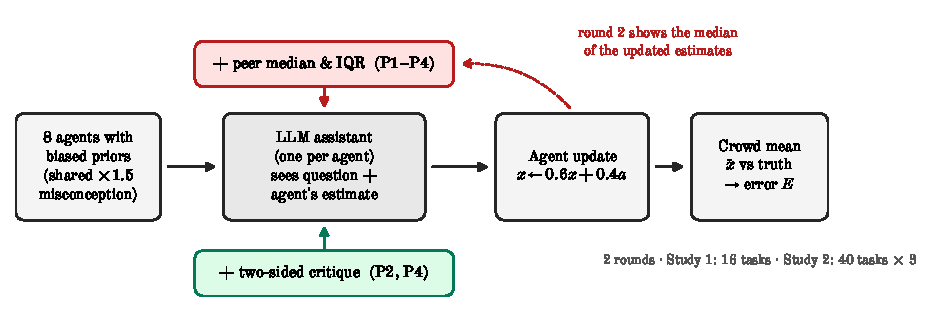
\includegraphics[width=0.8\linewidth]{fig0.pdf}
\captionsetup{type=figure}
\caption{Study design. Agents start from estimates biased in a shared direction. Each consults its own LLM assistant and moves 40\% of the way toward the assistant's answer. Conditions vary what the assistant sees (red) and whether it must first critique both anchors (green). P3/P4 replace six of the eight Gemma assistants with three other model families.}\label{fig:design}
\end{minipage}

\clearpage
\section{Introduction}
Imagine a panel of AI judges scoring a model's outputs, each shown the panel's running average before it votes. Every judgement still looks reasonable. But the panel may have quietly become a single judge. The same structure appears wherever AI assistants meet consensus signals: forecasters with live dashboards, analysts with shared spreadsheets, multi-agent pipelines that pass verdicts along. A second opinion is most valuable when its errors are independent of the first \citep{kleinberg2021,kim2025corr}, and this matters most when the consensus is stale, skewed or manufactured \citep{demarzo2003,denisov2026}.

Here is what this can look like. Eight agents believe, on average, that the Green Bank Telescope is about 1.5 times its true height of 148\,m. Each asks its own copy of the same AI assistant, Gemma-4-26B, for help. When each assistant sees only the agent it is helping, the crowd ends at 125\,m, 15\% below the truth. When the assistants also see the crowd's median, the same agents, starting from the same beliefs, end at 238\,m, 61\% above it (Study~1, Table~\ref{tab:tasks}; one of its largest effects, chosen to illustrate).

We set out to measure this failure, explain it and fix it, using numeric estimation because the truth is known. The story has a twist. Our discovery study found the effect, located most of it in one term of an exact accounting identity, and found a 53-word prompt that seemed to cure it completely. Before believing the cure, we committed a replication plan and ran it on 40 new tasks, with three replicates and three more model families. The effect grew stronger and appeared in all four model families; the cure shrank to a partial remedy. Along the way we found that pooled single-model baselines can favour mixing even without interaction.

Viewed as an evaluation, the setup probes what prior work calls \emph{epistemic independence} \citep{kelley2026}: whether a model keeps its own judgement when shown what others think. We report two group-level diagnostics: a same-direction error term from an exact accounting identity, and a variance-retention ratio (EVRR).

\paragraph{Contributions.}
\begin{enumerate}[leftmargin=*]
\item \textbf{Seeing the crowd makes assistants worse advisers, in every family tested.} Relative to the same model kept silent, final crowd error more than doubles for Gemma and DeepSeek and rises for Qwen, GLM and a four-model panel ($\pH\le0.003$ each; \S\ref{sec:repl}).
\item \textbf{Most of the added error points the same way twice.} In an exact accounting identity, the term for errors shared across rounds carries 56--69\% of the added error in every Study~2 panel decomposed. It describes where the error sits, not what causes it (\S\ref{sec:mech}, \S\ref{sec:mech2}).
\item \textbf{A two-sided critique helps, but only partly.} It beats length-matched generic reflection, though two-sidedness itself is not isolated, and error stays well above not showing the median (\S\ref{sec:repl}).
\item \textbf{Pooled single-model baselines do not isolate model interaction.} Comparing mixes with averaged single-model panels favours mixing by construction. A seat-matched comparison removes this bias for the interaction effect; by it, mixing helps only a little (\S\ref{sec:mix}, \S\ref{sec:jensen}).
\end{enumerate}

\smallskip\noindent Section~\ref{sec:setup} describes the setup, \S\ref{sec:results} the discovery study, \S\ref{sec:repl} the replication, \S\ref{sec:jensen} how to test model diversity fairly, and \S\ref{sec:meaning} what the results do and do not imply. Study~1's full request log is public; Study~2's raw logs are available on request, with SHA-256 digests in the repository (Appendix~\ref{app:code}).

\section{Related Work}
\textbf{Monoculture and correlated errors.} Shared algorithms can lower collective welfare even when each is individually better \citep{kleinberg2021}. LLM outputs are homogeneous across models \citep{jiang2025,qiu2026} (but see \citep{schaeffer2026}), AI-assisted writing loses diversity \citep{padmakumar2024,sourati2026}, and errors stay correlated across model families \citep{kim2025corr}, raising the prospect of knowledge collapse \citep{peterson2024}.

\textbf{Social influence and multi-LLM systems.} Double-counting shared signals produces persuasion bias even in rational updaters \citep{demarzo2003,goldman2001}, and in human crowds, seeing others' numerical estimates narrows their diversity and can undermine the wisdom-of-crowds effect \citep{lorenz2011}. LLM populations amplify majority errors and tip conventions \citep{ashery2025,centola2018,chuang2023,estornell2024,wynn2025}. Static cross-model aggregation rivals human forecasting crowds \citep{schoenegger2024,chuang2025}, and polling many models does not substitute for verification \citep{denisov2026}. Whether debate helps depends on how disagreement is structured \citep{quattrociocchi2025,schneider2025,smit2024,wang2024}.

\textbf{Cognitive forcing and sycophancy.} Making people commit before they see an anchor reduces over-reliance on AI \citep{bucinca2021}, and asking them to ``consider the opposite'' corrects biased judgement better than asking them to be unbiased \citep{lord1984}, a human analogue of our critique-versus-reflection comparison. LLMs do not self-correct without external structure \citep{huang2024}, can become stuck in incorrect solutions under self-reflection \citep{liang2024}, anchor to their own defaults in debate \citep{taubenfeld2024}, and defer to users \citep{sharma2024,deepthika2026,kelley2026,finnveden2024}. Closest to our setting, LLMs conform more to answers attributed to human experts than to other LLMs, even when the expert is wrong \citep{bajaj2026}, and sycophancy propagates through multi-agent discussion \citep{kasprova2026}. These studies measure answer changes on benchmarks; we measure numeric error against ground truth, decompose it exactly across rounds, and test a forcing prompt aimed at both the user's prior and the group consensus.

\Needspace{6\baselineskip}\section{Methods}\label{sec:setup}
\subsection{Simulation}
Each task $q$ has a positive ground truth $T_q$. We work in $\log_{10}$ space with target $y^\star=\log_{10}T_q$. There are $N=8$ \emph{agents}. Agents are not language models. Each holds a scalar estimate that moves a fixed step toward its own LLM \emph{assistant}'s answer:
\begin{equation}\label{eq:update}
x_{i,t}=(1-\alpha)\,x_{i,t-1}+\alpha\,a_{i,t},\qquad \alpha=0.4,\quad t\in\{1,2\}.
\end{equation}
Here $x_{i,t}$ and $a_{i,t}$ are log$_{10}$ estimates, $i$ indexes seats, and $t$ indexes rounds; task, replicate and condition indices are suppressed. A bar denotes the mean over the eight seats. If an answer cannot be parsed, the agent stays at $x_{i,t-1}$; for accounting we define its \emph{effective} answer as $a_{i,t}=x_{i,t-1}$. The assistant sees the question, the agent's current estimate and, in social conditions, the group's median and IQR (Fig.~\ref{fig:design}). The telemetry intervention bundles these statistics; it does not identify their separate effects. All language-model behaviour in this study is therefore the assistant's.

\paragraph{Biased priors by design.} Starting estimates are $x_{i,0}\sim\mathcal N(y^\star+0.22\,b_q,\;0.24^2)$ with $b_q=\pm0.8$. The group therefore shares a misconception that shifts it by a factor of about $1.5$ in a fixed direction per task. This models the threat of interest: a consensus signal that is systematically wrong. Priors are seeded and identical across conditions, so every between-condition difference comes from the assistants.

\subsection{Conditions}
\begin{table}[ht]\centering\small\setlength{\tabcolsep}{4.5pt}
\caption{Condition key. ``Mix'' = two assistants each of gemma-4-26b-a4b-it, deepseek-v4-flash, qwen3.8-27b and glm-5.2. Every arm ran in studies (Study~1: P0--P4 discovery run plus later controls; Study~2: three replicates).}\label{tab:cond}
\rowcolors{2}{gray!7}{white}
\begin{fittable}
\begin{tabular}{@{}llccl@{}}\toprule
Code & Assistants ($N=8$) & Sees crowd median & Extra prompt & Read as\\\midrule
P0 & 8$\times$ Gemma & no & --- & Gemma, silent\\
P1 & 8$\times$ Gemma & yes & --- & Gemma, median shown\\
P2 & 8$\times$ Gemma & yes & two-sided critique & Gemma, median + critique\\
P1\_REFLECT & 8$\times$ Gemma & yes & generic reflection & Gemma, median + reflection\\
P0\_X / P1\_X & 8$\times$ X (DS, QWEN, GLM) & no / yes & --- & one other model, silent / shown\\
P0\_POLY & mix & no & --- & mix, silent\\
P3 & mix & yes & --- & mix, median shown\\
P4 & mix & yes & two-sided critique & mix, median + critique\\\bottomrule
\end{tabular}
\end{fittable}
\end{table}

\noindent The \textbf{critique block} (53 words; Appendix~\ref{app:prompts}) asks the assistant, before answering, to name mechanisms by which \emph{both} the prior estimate and the peer median could overshoot \emph{or} undershoot, then to derive its estimate from independent principles. The harness omits temperature and top-p from its requests, leaving provider defaults in effect; response metadata may report the resolved values. It sets reasoning effort to \texttt{none} for DeepSeek, Qwen and GLM; the reasoning-effort field is omitted for Gemma. No Study~2 call reported separate reasoning tokens, which does not establish the absence of internal reasoning.

\subsection{Two studies}
\textbf{Study 1 (discovery).} 16 tasks selected from 24 pre-probed candidates within three strata, using each candidate's cold error, between-model disagreement and anchor sensitivity (Table~\ref{tab:tasks}); the selection was exploratory; one (LHC) was answered identically in all 80 calls and drops out of paired tests. One run per cell. Nine pairwise contrasts (Holm, $m=9$) and a $2\times2$ difference-in-differences were fixed in code before the run.

\textbf{Study 2 (replication).} 40 new quantities concerning 2025--2026, screened with a cold probe that removed items all models already recalled (model training cut-offs were not verified), with three replicates per cell and 13 arms: P0--P4, single-model panels of DeepSeek, Qwen and GLM with and without telemetry, a length-matched generic-reflection arm (P1\_REFLECT) and a silent four-model panel (P0\_POLY). Contrasts, Holm families ($m=4$ for P0--P4, $m=8$ for the controls), decision rules and a harness-equivalence margin ($\pm0.003$) were committed in git before the first Study~2 API call (\texttt{9ccd457}, 02:51 AEDT; cold probe 02:58; main run 03:08). This is a timestamped commitment, not an independent registry; deviations are listed in \texttt{REPORT.md} (Appendix~\ref{app:code}).

\textbf{Both studies.} The unit of analysis is the task (replicates averaged). The primary outcome is Round-2 crowd error $E_2=(\bar x_2-y^\star)^2$, tested with exact two-sided Wilcoxon signed-rank tests; for Study~2 we add post hoc paired bootstrap CIs (10,000 resamples), sign-flip permutation tests on the mean difference, and domain-clustered sensitivity analyses. These supplement the committed analysis plan and do not form additional confirmatory tests. For readability, Study~1 also reports transformed log RMSE, $100(10^{\sqrt{\overline E_2}}-1)$, where $\overline E_2$ averages tasks. Study~2 reports mean multiplicative deviation, $100(10^{|\bar x_2-y^\star|}-1)$ per run, averaged over replicates and tasks. These are different summaries; neither is ordinary absolute percentage error for underestimates.

\section{Study 1: A Clear Effect and an Apparent Cure}\label{sec:results}
We start with one model, Gemma-4-26B, and ask three questions in turn: does showing the median hurt (\S\ref{sec:herd}), can a prompt undo the harm (\S\ref{sec:rescue}), and why does it happen (\S\ref{sec:mech})?





\subsection{Seeing the median makes the crowd worse and its answers less varied}\label{sec:herd}
Adding the peer median and IQR raises mean Round-2 crowd error from 0.0119 (P0) to 0.0229 (P1), worse on 13 of 15 informative tasks (Table~\ref{tab:contrasts}, Appendix~\ref{app:s1}). Crowd diversity also falls 43\%. We summarise this with a variance-retention ratio, EVRR$_t=D_t/\big((1-\alpha)^2D_{t-1}\big)$, where $D_t=N^{-1}\sum_i(x_{i,t}-\bar x_t)^2$. Under Eq.~\eqref{eq:update}, if every assistant gave the same answer EVRR would equal 1, but the converse does not hold: other answer patterns can also give 1, so a value near 1 is consistent with, not proof of, convergence. EVRR drops from 1.38 (P0) to 1.07 (P1). Each assistant's behaviour shifts too. Its Round-2 answer tracks the crowd's Round-1 bias with slope $+0.45$ (P2: $-0.03$), while its sensitivity to the agent's own estimate falls from 0.134 to 0.009. In this sense the assistant attends less to the individual and more to the group.

The direction holds on all 16 leave-one-task-out subsets (uncorrected $p\le0.011$), but Holm-corrected significance was fragile here (it fails without Lake Superior, $\pH=0.064$). Study~2 provides stronger evidence (\S\ref{sec:repl}).

\subsection{An apparent cure: a two-sided critique}\label{sec:rescue}
Adding the critique block to the same model cuts crowd error by 48\% (0.0229 $\to$ 0.0118), improving 14 of 15 informative tasks. This survives every robustness check (Table~\ref{tab:robust}), and EVRR recovers to 1.34. P2's assistants wrote fewer output tokens on average than P1's (333 vs.\ 424), despite the additional input instructions; this is not a measurement of total compute.

P2's mean matched P0's ($-1\%$), but the 95\% CI ($[-0.0051,$ $+0.0044]$) is too wide to establish equivalence, and P2 was worse on 10 of 15 tasks. On 16 tasks and one run, it looked like a cure. Study~2 tested that.

\subsection{Why: errors that repeat across rounds}\label{sec:mech}
Averaging Eq.~\eqref{eq:update} gives $\bar x_2=0.6\,\bar x_1+0.4\,\bar a_2$, and hence exactly
\begin{equation}\label{eq:cross}
\begin{aligned}
E_2={}&\underbrace{0.36\,E_1}_{\text{carry-over}}
      +\underbrace{0.16\,(\bar a_2-y^\star)^2}_{\text{assistant error}}\\[3pt]
     &+\underbrace{0.48\,(\bar x_1-y^\star)(\bar a_2-y^\star)}_{\text{same-direction term}} .
\end{aligned}
\end{equation}
The last term is positive when the assistants err in the \emph{same direction} as the crowd already does. It is a product of signed errors, not a covariance: it is positive even for independent errors that share a bias. We use it as an accounting of where error sits, not as proof of a cause. It can be computed whenever ground truth eventually arrives.



The identity decomposes each condition exactly (Fig.~\ref{fig:mech} and Table~\ref{tab:cross}, Appendix~\ref{app:s1}). In P1 the same-direction term is $+0.0092$, 40\% of total error, against $+0.0034$ (28\%) in P0: Round 2 compounds Round 1 instead of correcting it. The critique cuts this term by 71\% (to $+0.0027$). It also accounts for why P4's crowd beat P3's although P4's assistants were \emph{less} accurate: the term fell from 0.0021 to 0.0007.

\paragraph{Robustness.} The critique and difference-in-differences contrasts hold under leave-one-task-out, corrected reference values, unit-error exclusion and two reconstructions of the original responses; the herding contrast does not survive the strictest reconstruction ($p=0.18$; Appendix~\ref{app:robust}).

\section{Study 2: The Effect Grows, the Cure Shrinks}\label{sec:repl}\label{sec:controls}
A single run on 16 tasks can flatter a result, so before trusting Study~1 we wrote down what would change our minds, committed it, and ran everything again. Study~2 repeats every condition on 40 new tasks with three replicates and adds the control arms (\S\ref{sec:setup}). All 24,960 cells completed; five answers (0.02\%, in four task-replicates) failed to parse and were kept unresampled, as pre-specified. Dropping those task-replicates changes one verdict (\S\ref{sec:mix}). The harness check passed (silent mixed vs.\ virtual panel: $+0.00006$, inside the $\pm0.003$ margin). Comparisons are against the silent arm: Gemma assistants shown the median still improved on the crowd's starting error on average (0.037 to 0.032), far less than silent ones (0.015), and left the crowd worse than it started on 8 of 40 tasks (2 when silent).

\begin{figure}[t]\centering
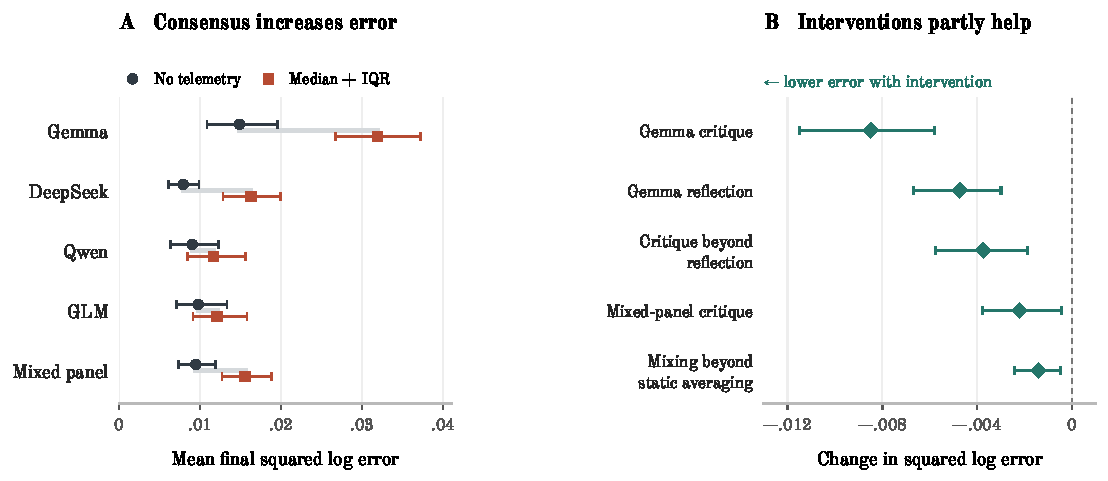
\includegraphics[width=\linewidth]{fig5.pdf}
\caption{\textbf{Study 2 on the primary outcome.} (A) Mean final squared log crowd error for each silent and social panel. (B) Paired changes from adding critique or reflection, critique versus generic reflection, and mixing versus its seat-matched virtual panel. Negative changes favour the named intervention. Points average three replicates within each of 40 tasks; whiskers are 95\% paired task-bootstrap percentile intervals (10,000 draws). These intervals are unadjusted; multiplicity-adjusted tests appear in Table~\ref{tab:repl}.}\label{fig:repl}
\end{figure}

\begin{table}[t]\centering\small\setlength{\tabcolsep}{3.6pt}
\caption{Study 2 contrasts specified in the committed plan on Round-2 crowd error (40 tasks; replicates averaged). $\Delta$: mean of (second $-$ first); W/L: tasks where the second-named arm is better/worse (no ties). CI: paired task-bootstrap 95\% interval for $\Delta$ (10,000 resamples). $\pH$: exact Wilcoxon, Holm-corrected within each family; sign-flip permutation tests on $\Delta$ and bootstraps clustered by task topic domain support the directions of the eight contrasts examined (Tables~\ref{tab:s2robust}--\ref{tab:s2extra}). Every contrast reaches the same verdict on the secondary metric $|\bar x_2-y^\star|$. Point estimates and Wilcoxon results reproduce the committed analysis; the additional sensitivity analyses are post hoc.}\label{tab:repl}
\rowcolors{2}{gray!7}{white}
\begin{fittable}
\begin{tabular}{@{}lrrccl@{}}\toprule
Contrast & $\Delta E_2$ & (rel.) & 95\% CI & W/L & $\pH$\\\midrule
\multicolumn{6}{@{}l}{\emph{P0--P4 family ($m=4$)}}\\
Herding, Gemma: P0 $\to$ P1 & $+0.0170$ & ($+115\%$) & $[+0.0124,+0.0219]$ & 4/36 & $<10^{-5}$\\
Critique, Gemma: P1 $\to$ P2 & $-0.0085$ & ($-27\%$) & $[-0.0115,-0.0058]$ & 35/5 & $<10^{-5}$\\
Critique, mixed panel: P3 $\to$ P4 & $-0.0022$ & ($-14\%$) & $[-0.0038,-0.0005]$ & 30/10 & $0.0009$\\
Mix + critique vs.\ silent Gemma: P0 $\to$ P4 & $-0.0015$ & ($-10\%$) & $[-0.0058,+0.0025]$ & 20/20 & $0.64$\\\midrule
\multicolumn{6}{@{}l}{\emph{Control family ($m=8$)}}\\
Herding, DeepSeek: P0\_DS $\to$ P1\_DS & $+0.0084$ & ($+106\%$) & $[+0.0061,+0.0108]$ & 1/39 & $<10^{-5}$\\
Herding, Qwen: P0\_QWEN $\to$ P1\_QWEN & $+0.0026$ & ($+29\%$) & $[+0.0016,+0.0038]$ & 8/32 & $2\times10^{-5}$\\
Herding, GLM: P0\_GLM $\to$ P1\_GLM & $+0.0023$ & ($+24\%$) & $[+0.0008,+0.0041]$ & 9/31 & $0.0025$\\
Herding, mixed panel: P0\_POLY $\to$ P3 & $+0.0061$ & ($+64\%$) & $[+0.0045,+0.0077]$ & 4/36 & $<10^{-5}$\\
Critique, mixed vs.\ silent mixed: P0\_POLY $\to$ P4 & $+0.0039$ & ($+41\%$) & $[+0.0023,+0.0057]$ & 6/34 & $2\times10^{-5}$\\
Generic reflection: P1 $\to$ P1\_REFLECT & $-0.0047$ & ($-15\%$) & $[-0.0067,-0.0030]$ & 32/8 & $<10^{-5}$\\
Critique vs.\ reflection: P1\_REFLECT $\to$ P2 & $-0.0037$ & ($-14\%$) & $[-0.0057,-0.0019]$ & 30/10 & $0.0005$\\
Beyond averaging: virtual social $\to$ P3 & $-0.0014$ & ($-8\%$) & $[-0.0024,-0.0005]$ & 26/14 & $0.011$\\\midrule
\multicolumn{6}{@{}l}{\emph{Best single model under telemetry ($m=2$; DeepSeek, chosen on its silent arm)}}\\
P1\_DS $\to$ P3 (mix) & $-0.0007$ & ($-4\%$) & $[-0.0025,+0.0010]$ & 19/21 & $0.79$\\
P1\_DS $\to$ P4 (mix + critique) & $-0.0029$ & ($-18\%$) & $[-0.0050,-0.0010]$ & 23/17 & $0.024$\\\bottomrule
\end{tabular}
\end{fittable}
\end{table}

\subsection{Herding replicates, and all four families do it}\label{sec:others}
Showing the median more than doubled Gemma's crowd error ($+115\%$, worse on 36 of 40 tasks), larger than in Study~1 and robust to adjusting all 14 planned contrasts together (Table~\ref{tab:repl}). Mean multiplicative deviation rose from 28\% to 47\%. DeepSeek, the most accurate model when silent, herded almost as hard ($+106\%$, worse on 39 of 40). Qwen ($+29\%$) and GLM ($+24\%$) herded least but still significantly, meeting the pre-registered rule that at least two of the three other families herd. The four-model panel herded too ($+64\%$). All five herding contrasts and both critique-versus-social contrasts remain significant after omitting any one task or topic domain and under a global Holm correction across all 14 planned contrasts (Appendix~\ref{app:sensitivity}). The replication supports effects that Study~1 did not resolve; the earlier nonsignificant results did not establish absence of an effect.

\subsection{The same-direction term replicates; loss of spread is not universal}\label{sec:mech2}
Eq.~\eqref{eq:cross} holds to $10^{-15}$ in all 1,560 Study~2 task--replicate--condition panels (Table~\ref{tab:decomp2}). Showing the median multiplied the same-direction term by $2.7\times$ for Gemma, $3.7\times$ for DeepSeek, $1.9\times$ for Qwen, $1.6\times$ for GLM and $2.3\times$ for the mix, and in every family it carried 56--69\% of the added error. The spread of effective assistant answers (carrying the prior forward on parse misses) fell by 77\% for Gemma, 42\% for GLM and 30\% for the mix, but barely for DeepSeek and Qwen ($-8\%$, $-7\%$, n.s.; Table~\ref{tab:s2extra}). Herding need not mean agreeing: DeepSeek's assistants moved toward the crowd together, keeping their spread.

\subsection{The critique helps, but only part of the way}\label{sec:reflect}
The critique cut Gemma's herded error by 27\% (35 of 40 tasks) and the mixed panel's by 14\%, with the same-direction term down 30\% and EVRR back to 1.42. Generic reflection of the same length helped too ($-15\%$), but the critique beat it on 30 of 40 tasks ($\pH=0.0005$). The two prompts differ in more than two-sidedness, so the gap cannot be credited to two-sidedness alone. Recovery was partial: the critique took back 50\% of Gemma's added error (post hoc 95\% paired-bootstrap CI: 37--67\%) and 37\% of the mix's (8--58\%; Appendix~\ref{app:sensitivity}). Gemma with the critique still missed by 38\% against 28\% when silent, and the mixed panel with the critique stayed 41\% worse than its silent version (6/34). Study~1's near-equal means did not replicate (Table~\ref{tab:glance}). The new tasks were harder, but the fraction recovered did not track task difficulty ($\rho=-0.09$; exploratory, Table~\ref{tab:s2extra}); this exploratory null association does not establish why the studies differ.

\subsection{Mixed panels: diversity helps a little, silence helps more}\label{sec:mix}
Mixing models did help beyond averaging. Against its seat-matched virtual twin (\S\ref{sec:pooled}), built from the same agents' single-model trajectories, the mixed panel's error was 8\% lower (26 of 40 tasks, $\pH=0.011$): the result is consistent with reduced herding under a cross-model consensus. With the critique added, the mix also beat herded DeepSeek, the model pre-specified as best on its silent arm ($-18\%$, 23 of 40 tasks, $\pH=0.024$; 0.06 without parse failures); without it, their difference was not statistically resolved ($\pH=0.79$). Herded Qwen had lower error than either (descriptive). But the gain is small next to the loss. The mixed panel still herded by $+64\%$, and silent DeepSeek alone was more accurate than the silent mix (typical miss 20\% vs.\ 22\%; descriptive).



\begin{table}[ht]\centering\small\setlength{\tabcolsep}{5pt}
\caption{The two studies at a glance (Gemma unless stated). Study~2 is larger and analysed under a committed plan; where they disagree, we give it greater weight.}\label{tab:glance}
\rowcolors{2}{gray!7}{white}
\begin{fittable}
\begin{tabular}{@{}lll@{}}\toprule
Question & Study 1 (16 tasks, 1 run) & Study 2 (40 tasks, 3 replicates)\\\midrule
Does showing the median hurt? & $+92\%$, $\pH=0.032$ (fragile) & $+115\%$, $\pH<10^{-5}$\\
Do other families herd? & same direction, n.s. & yes: DS $+106\%$, Qwen $+29\%$, GLM $+24\%$\\
Does the critique help? & $-48\%$, $\pH=0.001$ & $-27\%$, $\pH<10^{-5}$\\
Does it fully recover? & near-equal means; no equivalence test & no (P2 still $+58\%$ vs.\ P0)\\
Does it beat generic reflection? & inconclusive & yes ($\pH=0.0005$)\\
Does mixing help beyond averaging? & suggestive ($\pH=0.11$) & a little: $-8\%$, $\pH=0.011$\\
Does anything beat silence? & not significantly & silent arm has lowest mean in each panel\\\bottomrule
\end{tabular}
\end{fittable}
\end{table}

\FloatBarrier\clearpage
\section{A Baseline Trap When Testing Model Interaction}\label{sec:jensen}
Both studies leave one question open: when a panel mixes models, does it gain from their differences? Answering it needs care, because a pooled-baseline test favours ``yes''.


\Needspace{19\baselineskip}
\subsection{Diversity beyond chance}\label{sec:chance}
All variances below use the finite-panel divisor $N$, not $N-1$. These identities are deterministic; they require neither independent agents nor unbiased estimates.
\begin{proposition}[Hierarchical diversity--prediction identity]\label{prop:anova}
Partition the log estimates $z_1,\ldots,z_N$ into $K$ nonempty model families $G_k$ of sizes $n_k$, where $\sum_k n_k=N$. Write $\bar z=N^{-1}\sum_i z_i$ and $\bar z_k=n_k^{-1}\sum_{i\in G_k}z_i$. Let $E=(\bar z-y^\star)^2$ and $\bar e=N^{-1}\sum_i(z_i-y^\star)^2$. Then
\begin{equation}\label{eq:anova}
\begin{aligned}
E&=\bar e-\Dw-\Db,\\
\Dw&=\frac1N\sum_{k=1}^K\sum_{i\in G_k}(z_i-\bar z_k)^2,\qquad
\Db=\frac1N\sum_{k=1}^K n_k(\bar z_k-\bar z)^2.
\end{aligned}
\end{equation}
If $1\le K<N$, every $n_k=N/K$, and labels are assigned uniformly over balanced partitions conditional on the fixed estimates $z=(z_1,\ldots,z_N)$, then
\begin{equation}\label{eq:chance}
\E[\Db\mid z]=\frac{K-1}{N-K}\,\E[\Dw\mid z].
\end{equation}
\end{proposition}
\begin{proof}
Put $D=N^{-1}\sum_i(z_i-\bar z)^2$. Expanding $z_i-y^\star=(z_i-\bar z)+(\bar z-y^\star)$ and using $\sum_i(z_i-\bar z)=0$ gives $\bar e=D+E$, the ensemble ambiguity identity \citep{krogh1995,page2007}. Within group $k$, expand $z_i-\bar z=(z_i-\bar z_k)+(\bar z_k-\bar z)$; the cross term sums to zero because $\sum_{i\in G_k}(z_i-\bar z_k)=0$. Summing gives $D=\Dw+\Db$ and hence Eq.~\eqref{eq:anova}.

For random balanced groups, put $n=N/K>1$. Each group is a uniform sample without replacement. Using $\sum_{i<j}(z_i-z_j)^2=N^2D$, its sample variance satisfies
\[
\E[s_k^2\mid z]
=\frac{1}{n(n-1)}\frac{n(n-1)}{N(N-1)}
  \sum_{i<j}(z_i-z_j)^2=\frac{ND}{N-1},
\]
where $s_k^2=(n-1)^{-1}\sum_{i\in G_k}(z_i-\bar z_k)^2$ and $n(n-1)/(N(N-1))$ is the probability that a fixed pair belongs to the group. Thus
\[
\E[\Dw\mid z]=\frac{K(n-1)}{N}\frac{ND}{N-1}
=\frac{N-K}{N-1}D,\qquad
\E[\Db\mid z]=\frac{K-1}{N-1}D.
\]
Eliminating $D$ proves Eq.~\eqref{eq:chance}. No independence between groups is needed.
\end{proof}
\noindent With $N=8$ and $K=4$, random pairs already put $3/7$ of the variance between groups, so a positive $\Db$ on its own is not evidence of specialisation. We therefore report the excess over chance, \mbox{$\Dx=\Db-\frac34\Dw$}, and test it against all 105 pairings. In Study~1's mixed panels $\Dx$ is positive on average but significant on only 3/16 (P3) and 4/16 (P4) tasks.

\Needspace{19\baselineskip}
\subsection{Pooled baselines favour mixing by construction}\label{sec:pooled}

One possible baseline for a mixed panel is the \emph{average} performance of single-model panels of its constituent models. Our original analysis code used this comparison. It measures total ensemble benefit, but cannot by itself isolate an interaction benefit beyond static averaging.

\begin{proposition}[Static averaging in a pooled baseline]\label{prop:jensen}
Let family weights satisfy $w_k\ge0$ and $\sum_k w_k=1$. Suppose the mixed panel and its baseline use the \emph{same realised family-mean signed errors} $b_k$. With $\bar b_w=\sum_k w_kb_k$, define $E_{\mathrm{pool}}=\sum_k w_kb_k^2$ and $E_{\mathrm{mix}}=\bar b_w^2$. Then
\begin{equation}\label{eq:jensen}
E_{\mathrm{pool}}-E_{\mathrm{mix}}
=\sum_{k=1}^K w_k(b_k-\bar b_w)^2\ge0.
\end{equation}
Equality holds exactly when all positive-weight families have the same signed error. Equal allocation corresponds to $w_k=1/K$.
\end{proposition}
\begin{proof}
Expanding the right-hand side gives $\sum_k w_kb_k^2-2\bar b_w\sum_k w_kb_k+\bar b_w^2\sum_k w_k=E_{\mathrm{pool}}-\bar b_w^2$. Each summand is nonnegative; the sum is zero precisely under the stated equality condition.
\end{proof}
\noindent The gap is the weighted between-family variance: Jensen's inequality, or the ensemble ambiguity identity applied one level up. This elementary result explains why a pooled baseline can credit static averaging to interaction. Its matched-mean assumption matters: a two-seat subset need not have its eight-seat source panel's mean, and independent model calls add noise. The theorem therefore does \emph{not} guarantee a nonnegative gap in every empirical mixed-versus-pooled comparison.

\paragraph{Seat-matched virtual panels.} The fix uses the fact that each agent's seeded prior is identical across conditions. For every seat in the mixed panel, take \emph{the same agent's} trajectory from the single-model arm of that seat's family, and recompute the crowd error from those eight trajectories. Both sides now use the same seat allocation and aggregation rule. Subject to matched execution settings and sampling noise, mixed minus virtual estimates what mixing changes beyond averaging: here, the effect of seeing a cross-model median instead of a single-model one. It also gives a free harness check: silent agents never interact, so silent mixed and virtual panels must agree up to noise.

\paragraph{Executable checks.} The supplement checks these identities with exact rational arithmetic, including all 105 pairings of eight seats. These checks validate the algebra; they do not estimate the virtual-panel test's false-positive rate (Appendix~\ref{app:math}).



\paragraph{On the real data.} In Study~1 the pooled and seat-matched contrasts almost coincided ($-0.00296$ vs.\ $-0.00295$). In Study~2 the silent version passed the harness check, and the social version found a modest benefit of mixing ($-8\%$, $\pH=0.011$; \S\ref{sec:mix}); correcting all 14 contrasts together gives $p=0.044$ (Appendix~\ref{app:sensitivity}). Neither comparison establishes the test's calibration under arbitrary response dependence.

\section{Discussion and Limitations}\label{sec:meaning}
\subsection{Recommendations}
Read together, the two studies tell a simple story: consensus aligns assistants' errors with the crowd's across rounds, usually narrowing their answers too, and talking them out of it works only part of the way. Four practical lessons follow. (1)~\textbf{Preserve a no-telemetry baseline when consensus may be biased.} In Study~2, the panel that never saw the median was the most accurate in every family. (2)~\textbf{Evaluate structured critique when an assistant must see potentially biased consensus.} The 53-word protocol beat generic reflection and recovered about half of Gemma's added error in Study~2. Total compute was not measured. Its value when consensus is accurate remains untested (Appendix~\ref{app:ethics}). (3)~\textbf{Monitor the same-direction term} (Eq.~\ref{eq:cross}) and EVRR. Both are cheap; the first needs eventual ground truth. (4)~\textbf{Do not assume a mix of models resists herding.} Ours herded by $+64\%$; a cross-model median herded only 8\% less than same-model ones. Where mixing is the claim, test it against seat-matched virtual panels.

\subsection{Implications for AI oversight}\label{sec:oversight}
Panels of AI judges, monitor ensembles and debate protocols draw their value from independent errors \citep{kim2025corr,estornell2024,smit2024}. Showing each judge the panel's running verdict could make their errors line up in a way no review of single outputs is designed to catch; the same-direction term could flag it once ground truth arrives. Withholding the running verdict is a candidate design to test against social panels, especially when consensus may be biased. The experiments reported here do not test judging tasks, so this is a hypothesis, not a finding.

\subsection{Limitations}\label{sec:lim}
Appendix~\ref{sec:cruxes} grades every claim by the strength of its evidence.
\begin{enumerate}
\item \textbf{Comparator}: harm is relative to silent assistants; assistants shown the median still improve on the crowd's starting estimates on average (not on 8 of 40 tasks).
\item \textbf{Accounting, not mechanism}: Eq.~\ref{eq:cross} and EVRR describe where error sits and how spread changes; neither identifies a cause.
\item \textbf{Scope}: simulated fixed-$\alpha$ agents, selected numeric tasks, provider-default temperature, one wording each for telemetry and critique, and no one-sided critique ablation.
\item \textbf{Recovery differs between studies}: near-equal means in Study~1, partial recovery in Study~2; the reason remains unresolved, and we give greater weight to the larger study.
\end{enumerate}

\subsection{Future Work}\label{sec:future}
Next: ablate one-sided against two-sided critique, add conditions where the consensus is accurate, and move to a real panel of AI judges shown its running verdict, with reasoning on.

\section{Conclusion}
Sharing one number can erode the independence that makes a second opinion useful. In our biased-prior numerical tasks, showing peer statistics raised final crowd error in every tested family, by up to $2.1\times$ relative to withholding those statistics. A 53-word critique recovered about half of Gemma's added error and about a third of the mixed panel's. Independent estimation was the strongest baseline within each tested panel composition; transfer to other settings remains open.

\section*{Code and Data}
Code, analysis outputs and Study~1 request logs: \url{https://github.com/vikramwish/apart-epistemics} (details in Appendix~\ref{app:code}). Study~1 numbers are regenerated by \texttt{scripts/audit\_and\_reproduce\_p0\_p4.py} from the frozen run log (the Page identity holds to $2\times10^{-16}$ in all 320 cells); Study~2 numbers by the locked functions in \texttt{scripts/analyze\_controls\_preregistered.py}.

\section*{Author Contributions}
V.V.\ designed the study, built the harness and diagnostics, ran all experiments and audits, and wrote the paper. Kevin O'Shaughnessy contributed harness code during the sprint: numeric parsing, provider backends and retries, concurrency and budget handling, command-line run options, and the H4 slope computation.

\small
\clearpage
\begingroup\raggedright
\begin{thebibliography}{35}
\bibitem{ashery2025} A.~F. Ashery, L.~M. Aiello, A.~Baronchelli. Emergent social conventions and collective bias in LLM populations. \emph{Science Advances} 11(20):eadu9368, 2025.
\bibitem{bajaj2026} A.~Bajaj, Z.~Tiganj. Who do LLMs trust? Human experts matter more than other LLMs. \href{https://arxiv.org/abs/2602.13568}{arXiv:2602.13568}, 2026.
\bibitem{bucinca2021} Z.~Bu\c{c}inca, M.~B. Malaya, K.~Z. Gajos. To trust or to think: Cognitive forcing functions can reduce overreliance on AI in AI-assisted decision-making. \emph{Proc.\ ACM HCI} 5(CSCW1), 2021.
\bibitem{centola2018} D.~Centola, J.~Becker, D.~Brackbill, A.~Baronchelli. Experimental evidence for tipping points in social convention. \emph{Science} 360:1116--1119, 2018.
\bibitem{chuang2023} Y.-S. Chuang et al. Simulating opinion dynamics with networks of LLM-based agents. arXiv:2311.09618, 2023.
\bibitem{chuang2025} Y.-S. Chuang et al. Probing LLM world models: Enhancing guesstimation with wisdom of crowds decoding. \emph{EMNLP}, pp.~4699--4713, 2025.
\bibitem{deepthika2026} Deepthika S, P.~Yadav, B.~Sankar. Who is sycophantic to whom? Confident LLMs, human deference, and the collapse of trust calibration. arXiv preprint, October 2026.
\bibitem{demarzo2003} P.~M. DeMarzo, D.~Vayanos, J.~Zwiebel. Persuasion bias, social influence, and unidimensional opinions. \emph{QJE} 118(3):909--968, 2003.
\bibitem{denisov2026} Y.~Denisov-Blanch, J.~Kazdan, J.~Chudnovsky, R.~Schaeffer, S.~Guan, S.~Adeshina, S.~Koyejo. Truthfulness does not scale like reasoning: Why polling fails as a proxy verifier. \emph{ICML}, \href{https://proceedings.mlr.press/v306/denisov-blanch26a.html}{PMLR 306:24461--24477}, 2026. (arXiv:2603.06612: ``Consensus is not verification'').
\bibitem{estornell2024} A.~Estornell, Y.~Liu. Multi-LLM debate: Framework, principals, and interventions. \emph{NeurIPS}, 2024.
\bibitem{finnveden2024} L.~Finnveden. What's important in ``AI for epistemics''? Forethought research note, 2024.
\bibitem{goldman2001} A.~I. Goldman. Experts: Which ones should you trust? \emph{Phil.\ Phenomenol.\ Res.} 63(1):85--110, 2001.
\bibitem{huang2024} J.~Huang et al. Large language models cannot self-correct reasoning yet. \emph{ICLR}, 2024.
\bibitem{jiang2025} L.~Jiang et al. Artificial hivemind: The open-ended homogeneity of language models (and beyond). arXiv:2510.22954, 2025.
\bibitem{kasprova2026} V.~Kasprova, A.~Parulekar, A.~AlRabah, K.~Agaram, R.~Garg, S.~Jha, N.~B. Bozdag, D.~Hakkani-T\"ur. Too polite to disagree: Understanding sycophancy propagation in multi-agent systems. \emph{SIGDIAL}, pp.~795--814, 2026. \href{https://arxiv.org/abs/2604.02668}{arXiv:2604.02668}.
\bibitem{kelley2026} S.~W. Kelley, C.~Riedl. Personalization increases affective alignment but has role-dependent effects on epistemic independence in LLMs. arXiv:2603.00024, 2026.
\bibitem{kim2025corr} E.~M. Kim, A.~Garg, K.~Peng, N.~Garg. Correlated errors in large language models. \emph{ICML}, \href{https://proceedings.mlr.press/v267/kim25e.html}{PMLR 267:30038--30066}, 2025.
\bibitem{kleinberg2021} J.~Kleinberg, M.~Raghavan. Algorithmic monoculture and social welfare. \emph{PNAS} 118(22), 2021.
\bibitem{krogh1995} A.~Krogh, J.~Vedelsby. Neural network ensembles, cross validation, and active learning. \emph{NIPS 7}, 1995.
\bibitem{lord1984} C.~G. Lord, M.~R. Lepper, E.~Preston. Considering the opposite: A corrective strategy for social judgment. \emph{J.\ Personality and Social Psychology} 47(6):1231--1243, 1984.
\bibitem{lorenz2011} J.~Lorenz, H.~Rauhut, F.~Schweitzer, D.~Helbing. How social influence can undermine the wisdom of crowd effect. \emph{PNAS} 108(22):9020--9025, 2011.
\bibitem{liang2024} T.~Liang et al. Encouraging divergent thinking in large language models through multi-agent debate. \emph{EMNLP}, pp.~17889--17904, 2024. \href{https://aclanthology.org/2024.emnlp-main.992/}{doi:10.18653/v1/2024.emnlp-main.992}.
\bibitem{padmakumar2024} V.~Padmakumar, H.~He. Does writing with language models reduce content diversity? \emph{ICLR}, 2024.
\bibitem{page2007} S.~E. Page. \emph{The Difference}. Princeton University Press, 2007.
\bibitem{peterson2024} A.~J. Peterson. AI and the problem of knowledge collapse. \emph{AI \& Society}, 2024.
\bibitem{qiu2026} Z.~Qiu, R.~Hu, Y.~Ding, T.~Underwood. Revisiting LLM homogeneity through a multidimensional lens. arXiv:2611.01549, 2026.
\bibitem{quattrociocchi2025} W.~Quattrociocchi, V.~Capraro, M.~Perc. Epistemological fault lines between human and artificial intelligence. arXiv:2512.19466, 2025.
\bibitem{schaeffer2026} R.~Schaeffer, B.~Miranda, J.~Kazdan, J.~Chudnovsky, S.~Koyejo. How strong is the evidence for the artificial hivemind? Reevaluating evidence for the open-ended homogeneity of language models. arXiv:2609.33936, 2026.
\bibitem{schneider2025} P.~Schneider, A.~Schramm. The wisdom of deliberating AI crowds: Does deliberation improve LLM-based forecasting? arXiv:2512.22625, 2025.
\bibitem{schoenegger2024} P.~Schoenegger et al. Wisdom of the silicon crowd: LLM ensemble prediction capabilities rival human crowd accuracy. \emph{Science Advances} 10(45), 2024.
\bibitem{sharma2024} M.~Sharma et al. Towards understanding sycophancy in language models. \emph{ICLR}, 2024.
\bibitem{smit2024} A.~Smit et al. Should we be going MAD? A look at multi-agent debate strategies for LLMs. \emph{ICML}, 2024.
\bibitem{sourati2026} Z.~Sourati et al. The shrinking landscape of linguistic diversity in the age of large language models. \emph{Nature Human Behaviour}, 2026. doi:10.1038/s41562-026-02550-0.
\bibitem{taubenfeld2024} A.~Taubenfeld et al. Systematic biases in LLM simulations of debates. \emph{EMNLP}, 2024.
\bibitem{wang2024} J.~Wang et al. Mixture-of-agents enhances large language model capabilities. arXiv:2406.04692, 2024.
\bibitem{wynn2025} A.~Wynn, H.~Satija, G.~K. Hadfield. Talk isn't always cheap: Understanding failure modes in multi-agent debate. ICML Workshop on Multi-Agent Systems, 2025. arXiv:2509.05396.
\end{thebibliography}
\endgroup
\normalsize

\appendix
\clearpage
\section{Code and Data Availability}\label{app:code}
\textbf{Pre-existing work.} None. All code, configuration, prompts, task sets and analysis scripts were written during the sprint (13--16 November 2026). An early exploratory direction, \path{propaganda-eval/}, is not part of the current paper repository or the reported experiments.

Code, configuration, analysis outputs and Study~1 run archives are available at \url{https://github.com/vikramwish/apart-epistemics} (branch \texttt{numeric-question-bank}). Study~1 (P0--P4) is frozen at commit \texttt{3a6294c}; the control-arm harness is at commit \texttt{5ad9f34}. Study~2's analysis plan and code were first committed at \texttt{3d41492} (02:42 AEDT, 16 Nov 2026, controls plan) and extended for the replication at \texttt{9ccd457} (02:51); the first Study~2 API call was a screening cold probe at 02:58, and the main run began at 03:08. Deviations from the plan, listed in \texttt{REPORT.md} \S4: the cold-probe prompt was reconstructed because the original was not saved; the budget-reservation settings differed from the plan; and after a provider outage the run was resumed with fewer workers and an owner-authorised budget-cap increase, with an unchanged manifest. SHA-256 digests for the raw logs are recorded in \texttt{PROVENANCE.md}. Its outputs (\texttt{REPORT.md}, \texttt{PROVENANCE.md}, \texttt{preregistered\_analysis.json}, the integrity audit and the task file) are on branch \texttt{replication-2025} at commit \texttt{d09862d}. The raw run logs (\texttt{numeric\_runs.jsonl}, 637\,MB; \texttt{provider\_requests.jsonl}, 166\,MB) exceed GitHub's file limit; their SHA-256 digests are in \texttt{PROVENANCE.md}, and the files are available on request.

\begin{itemize}
\item \textbf{Raw request log:} every one of the 1,318 HTTP calls, including the 38 not analysed: \path{results/polyphony-p0-p4/provider_requests.jsonl}.
\item \textbf{Frozen records:} \path{results/polyphony-p0-p4/numeric_runs.jsonl}. Analysis output: \path{numeric_analysis.json} in the same directory.
\item \textbf{Audit and reproduction:} \path{scripts/audit_and_reproduce_p0_p4.py} regenerates every reported number from the frozen log.
\item \textbf{Study 2 committed analysis and virtual panels:} \path{scripts/analyze_controls_preregistered.py}. Post hoc sensitivity analyses and revised figures: \path{reports/manuscript/}; see its README for reproduction commands and the supplied-source provenance.
\item \textbf{Task definitions and controls:} \path{configs/polyphony_benchmark_tasks.json}, \path{configs/polyphony_controls.yaml}.
\end{itemize}

\section{Limitations and Dual-Use / Ethical Considerations}\label{app:ethics}
\textbf{What the result does and does not establish.} With simulated scalar agents, it establishes that showing the crowd median makes assistants worse advisers than silent ones in all four model families tested, with most of the added error in the same-direction term, and that a two-sided critique reduces but does not remove the effect, more than generic reflection does. It also finds that a cross-model median herds slightly less than a same-model one. It does not establish a causal mechanism, that two-sidedness is the active ingredient, that assistants make crowds worse than they started, or that any of this transfers to human users, to real judging tasks, or to models with reasoning modes on. Limitations are listed in \S\ref{sec:lim}; Appendix~\ref{sec:cruxes} grades every claim.

\textbf{Manufactured consensus.} Anyone who controls the aggregator an assistant reads from could inject a skewed median and steer an AI-assisted crowd. Our P1 condition shows the underlying susceptibility, not an attack: we did not test an adversarial aggregator, a deliberately tightened IQR or refusal behaviour. Possible mitigations, all untested: treat consensus telemetry as untrusted input, have the assistant commit to an independent estimate before it sees consensus, and alert on a rising same-direction term once ground truth is available.

\textbf{Weaponised doubt.} The opposite misuse is indiscriminate anti-consensus prompting that erodes correct agreement. Gemma's error \emph{rose} in P4 when it was asked to critique stronger peers (Fig.~\ref{fig:mech}, right). Whether gating critique on evidence of herding improves outcomes requires a separate experiment.

\textbf{Research ethics.} No human subjects; no personal data was collected, stored or processed. All tasks use public institutional figures (EIA, CERN, IPCC, NIST, EPA, RTE, ESO, MDBA, NRAO, SNOLAB). Study~1 cost \$0.50 and Study~2 \$17.28. No credentials are committed.

\section{Tasks and Per-Task Results}
\begin{table}[ht]\centering\scriptsize\setlength{\tabcolsep}{3.5pt}
\caption{All 16 tasks with Round-2 crowd error $E_2$. Strata: HS high-spread, LS low-spread, C control. $b_q$: direction of the injected misconception.}\label{tab:tasks}
\rowcolors{2}{gray!7}{white}
\begin{fittable}
\begin{tabular}{@{}llrlr ccccc@{}}\toprule
Task & Str. & Truth & Source & $b_q$ & P0 & P1 & P2 & P3 & P4\\\midrule
US hydro 2023 & HS & 240 TWh & US EIA & $-$ & .01881 & .00869 & .00416 & .00388 & .00226\\
LHC dipole magnets & HS & 1,232 & CERN & $-$ & .01679 & .01679 & .01679 & .01679 & .01679\\
P\"aij\"anne tunnel & HS & 120 km & HSY & $+$ & .00692 & .01247 & .00845 & .01394 & .01067\\
Green Bank Telescope height & HS & 148 m & NRAO & $+$ & .00524 & .04271 & .02778 & .00706 & .00158\\
Delaware Aqueduct & HS & 137 km & NYC DEP & $+$ & .02029 & .04698 & .02446 & .01363 & .00852\\
France nuclear 2022 & HS & 279 TWh & RTE & $-$ & .00002 & .00179 & .00104 & .00276 & .00604\\
ELT collecting area & LS & 978 m$^2$ & ESO & $+$ & .00332 & .00284 & .00164 & .00119 & .00089\\
Molybdenum melting pt. & LS & 2,623 $^\circ$C & NIST/CRC & $-$ & .01276 & .01478 & .01309 & .01331 & .01247\\
US wind 2023 & LS & 425 TWh & US EIA & $+$ & .01042 & .05410 & .02138 & .02278 & .01201\\
Norway hydro 2023 & LS & 136 TWh & US EIA Intl. & $+$ & .00399 & .01615 & .00534 & .00692 & .00547\\
Murray--Darling area & LS & 1,061,469 km$^2$ & MDBA/BoM & $-$ & .00568 & .00601 & .00607 & .00452 & .00412\\
CH$_4$ in 1750 (IPCC) & LS & 729 ppb & IPCC AR6 & $-$ & .00230 & .00262 & .00216 & .00263 & .00231\\
US nuclear 2023 & C & 775 TWh & US EIA & $+$ & .00428 & .00793 & .00326 & .00425 & .00347\\
Lake Superior volume & C & 12,100 km$^3$ & EPA/NOAA & $-$ & .06209 & .10245 & .03434 & .03211 & .01757\\
SNOLAB depth & C & 2,070 m & SNOLAB & $-$ & .00934 & .01488 & .00965 & .00872 & .01341\\
North Sea Link & C & 720 km & Nat.\ Grid/Statnett & $+$ & .00890 & .01522 & .00950 & .00646 & .00552\\\midrule
\textbf{Mean} &&&&& \textbf{.01194} & \textbf{.02290} & \textbf{.01182} & \textbf{.01006} & \textbf{.00769}\\\bottomrule
\end{tabular}
\end{fittable}
\end{table}

\begin{table}[ht]\centering\small
\caption{Full diversity decomposition (agents). $E_a=(\bar a-y^\star)^2$ is the squared error of the mean assistant log estimate; all entries average task-level quantities. $E=\bar e-\Dw-\Db$ holds to $2\times10^{-16}$. EVRR $=D_t/\big((1-\alpha)^2D_{t-1}\big)$, averaged over tasks: identical assistant answers give 1, but other answer patterns can too, so values are descriptive. P1's 1.07 in Round 2 is the lowest of the five conditions.}\label{tab:div}
\begin{fittable}
\begin{tabular}{@{}llcccccccc@{}}\toprule
Cond. & Rnd & $E$ & $\bar e$ & $D$ & $\Dw$ & $\Db$ & $\Dx$ & $E_a$ & EVRR\\\midrule
P0 & R1 & .01952 & .04808 & .02856 & .02856 & 0 & 0 & .01913 & 1.28\\
P0 & R2 & .01194 & .02875 & .01681 & .01681 & 0 & 0 & .00965 & 1.38\\
P1 & R1 & .03027 & .05557 & .02530 & .02530 & 0 & 0 & .01903 & 1.12\\
P1 & R2 & .02290 & .03246 & .00956 & .00956 & 0 & 0 & .01731 & 1.07\\
P2 & R1 & .01935 & .04482 & .02548 & .02548 & 0 & 0 & .02289 & 1.16\\
P2 & R2 & .01182 & .02467 & .01285 & .01285 & 0 & 0 & .01348 & 1.34\\
P3 & R1 & .02111 & .04401 & .02290 & .01142 & .01148 & .00292 & .00402 & 1.06\\
P3 & R2 & .01006 & .01908 & .00902 & .00418 & .00484 & .00171 & .00234 & 1.11\\
P4 & R1 & .01696 & .04294 & .02598 & .01082 & .01516 & .00705 & .00415 & 1.12\\
P4 & R2 & .00769 & .02153 & .01384 & .00484 & .00901 & .00538 & .00577 & 1.28\\\bottomrule
\end{tabular}
\end{fittable}
\end{table}

\begin{table}[ht]\centering\small
\caption{Exact cross-round decomposition of $E_2$ (Eq.~\ref{eq:cross}).}\label{tab:cross}
\begin{fittable}
\begin{tabular}{@{}lcccc c@{}}\toprule
Cond. & $0.36E_1$ & $0.16E_{a,2}$ & Same-direction term & $E_2$ & Term share\\\midrule
P0 & .00703 & .00154 & +.00337 & .01194 & 28\%\\
P1 & .01090 & .00277 & +.00923 & .02290 & 40\%\\
P2 & .00697 & .00216 & +.00270 & .01182 & 23\%\\
P3 & .00760 & .00037 & +.00209 & .01006 & 21\%\\
P4 & .00611 & .00092 & +.00066 & .00769 & 9\%\\\bottomrule
\end{tabular}
\end{fittable}
\end{table}

\FloatBarrier
\section{Study 1 Results in Detail}\label{app:s1}
\begin{figure}[ht]\centering
\begin{minipage}{0.35\linewidth}\centering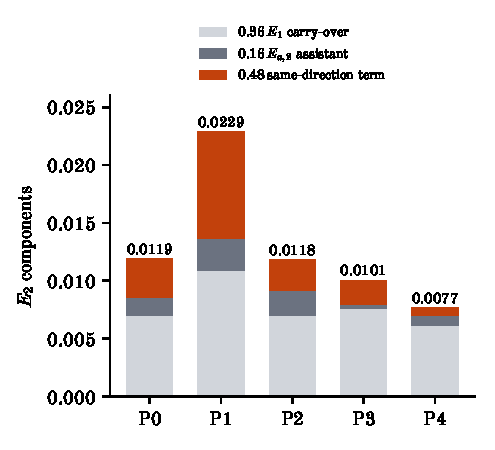
\includegraphics[width=\linewidth]{fig2.pdf}\end{minipage}\hfill
\begin{minipage}{0.32\linewidth}\centering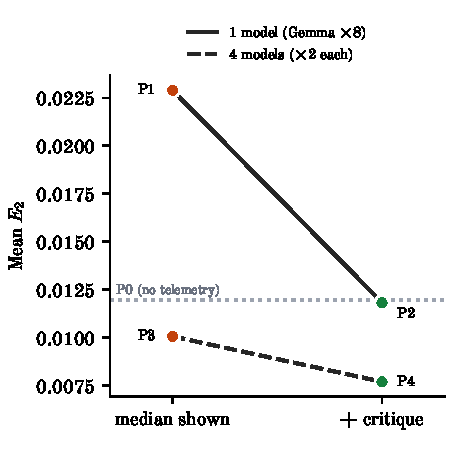
\includegraphics[width=\linewidth]{fig3.pdf}\end{minipage}\hfill
\begin{minipage}{0.32\linewidth}\centering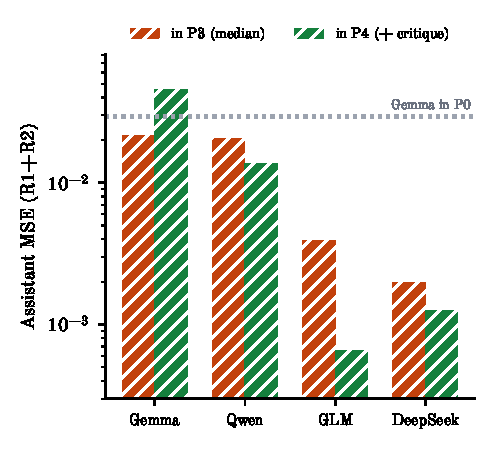
\includegraphics[width=\linewidth]{fig4.pdf}\end{minipage}
\caption{\textbf{Left:} exact split of $E_2$ (Eq.~\ref{eq:cross}). Study~1. The same-direction term (red) is what telemetry inflates in P1 and the critique shrinks in P2/P4. \textbf{Middle:} the interventions overlap. Critique helps a lot in the single-model panel and little in the mixed one. \textbf{Right:} the capability confound. Two of the three replacement models have about 10$\times$ lower error than Gemma.}\label{fig:mech}
\end{figure}
\begin{figure}[ht]\centering
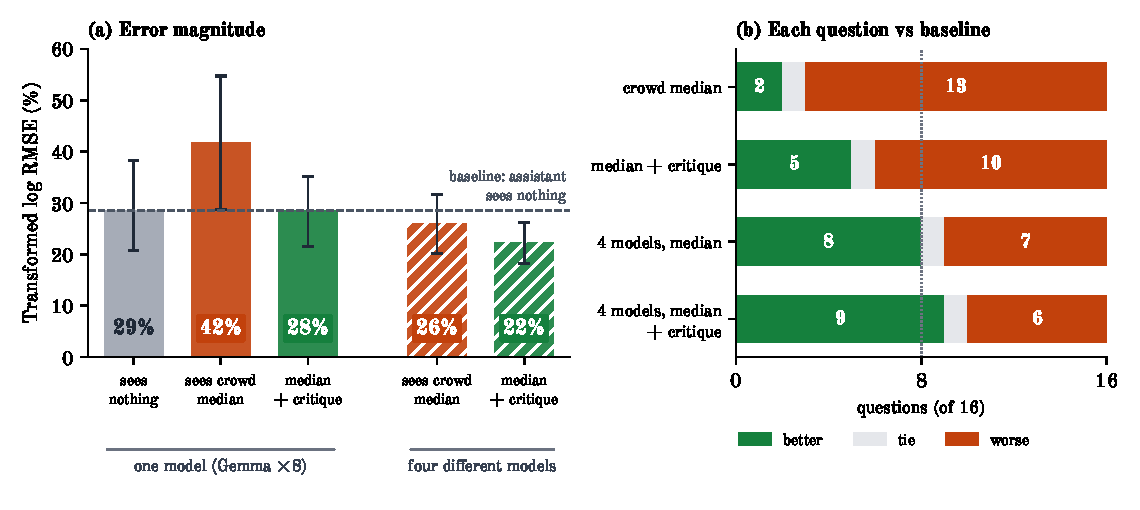
\includegraphics[width=\linewidth]{fig1.pdf}
\caption{\textbf{Study 1: telemetry raises error; critique brings the mean close to baseline without establishing equivalence.} \textbf{(a)}~Transformed task-mean log RMSE, $100(10^{\sqrt{\overline E_2}}-1)$, over 16 questions; error bars transform the task-bootstrap 95\% intervals for mean $E_2$. Showing the assistant the crowd median raises this summary from 29\% to 42\%. Adding the two-sided critique brings it back to 28\%. Four-model panels (hatched) do slightly better still, but not significantly better than showing nothing. \textbf{(b)}~On how many of the 16 questions each condition beat the baseline. Even with the critique, the single-model panel is worse than showing nothing on 10 questions. Statistics use squared log error; per-question values are in Table~\ref{tab:tasks}.}\label{fig:main}
\end{figure}
\begin{table}[ht]\centering\small\setlength{\tabcolsep}{4pt}
\caption{Study 1 pre-specified contrasts on Round-2 crowd error ($n=16$; LHC tied throughout). W/L: tasks where the first-named condition is better/worse. $p$: exact Wilcoxon; $\pH$: Holm ($m=9$ pairwise; $m=5$ for DiD).}\label{tab:contrasts}
\rowcolors{2}{gray!7}{white}
\begin{fittable}
\begin{tabular}{@{}llrcccc@{}}\toprule
Question & Contrast & $\Delta E_2$ (rel.) & 95\% CI & W/L & $p$ & $\pH$\\\midrule
Does telemetry hurt? & P1 vs P0 & $+0.0110$ ($+92\%$) & $[+0.0037,+0.0191]$ & 2/13 & 0.0054 & \textbf{0.032}\\
Does critique fix it? & P2 vs P1 & $-0.0111$ ($-48\%$) & $[-0.0203,-0.0042]$ & 14/1 & 0.0001 & \textbf{0.001}\\
Does mixing fix it? & P3 vs P1 & $-0.0128$ ($-56\%$) & $[-0.0231,-0.0045]$ & 12/3 & 0.0012 & \textbf{0.009}\\
Both together & P4 vs P1 & $-0.0152$ ($-66\%$) & $[-0.0276,-0.0051]$ & 14/1 & 0.0012 & \textbf{0.009}\\
Critique on top of mixing & P4 vs P3 & $-0.0024$ ($-24\%$) & $[-0.0048,-0.0003]$ & 13/2 & 0.026 & 0.128\\
Mixing on top of critique & P4 vs P2 & $-0.0041$ ($-35\%$) & $[-0.0086,-0.0005]$ & 9/6 & 0.151 & 0.606\\
\emph{Beats no telemetry?} & P4 vs P0 & $-0.0043$ ($-36\%$) & $[-0.0109,+0.0005]$ & 9/6 & 0.389 & 1.000\\
& P2 vs P0 & $-0.0001$ ($-1\%$) & $[-0.0051,+0.0044]$ & 5/10 & 0.454 & 1.000\\\midrule
Do effects add? & DiD & $+0.0087$ & $[+0.0035,+0.0158]$ & --- & 0.0002 & \textbf{0.0009}\\\bottomrule
\end{tabular}
\end{fittable}
\end{table}

\FloatBarrier
\clearpage
\section{Study 2 Decomposition}\label{app:s2}
\begin{table}[ht]\centering\small\setlength{\tabcolsep}{5pt}
\caption{Study 2 exact decomposition of Round-2 crowd error (Eq.~\ref{eq:cross}; 40 tasks, replicates averaged within task) and variance-retention ratio (EVRR). The three terms sum to $E_2$ to within $10^{-15}$ per task--replicate--condition panel. One Round-2 assistant call failed to parse in each of P0\_POLY, P3 and P4; there the agent kept its estimate, and $\bar a_2$ uses that value so that $\bar x_2=0.6\bar x_1+0.4\bar a_2$ holds exactly. Recomputed independently from the raw log.}\label{tab:decomp2}
\rowcolors{2}{gray!7}{white}
\begin{fittable}
\begin{tabular}{@{}lrrrrrr@{}}\toprule
Arm & $0.36E_1$ & $0.16(\bar a_2-y^\star)^2$ & same-dir. & $E_2$ & share & EVRR$_2$\\\midrule
P0 & 0.00753 & 0.00175 & $+$0.00559 & 0.01487 & 38\% & 1.87\\
P1 & 0.01189 & 0.00492 & $+$0.01509 & 0.03191 & 47\% & 1.19\\
P2 & 0.00966 & 0.00323 & $+$0.01054 & 0.02343 & 45\% & 1.42\\
P1\_REFLECT & 0.01069 & 0.00392 & $+$0.01256 & 0.02717 & 46\% & 1.22\\
P0\_DS & 0.00555 & 0.00059 & $+$0.00178 & 0.00792 & 22\% & 1.35\\
P1\_DS & 0.00795 & 0.00169 & $+$0.00663 & 0.01627 & 41\% & 1.17\\
P0\_QWEN & 0.00609 & 0.00083 & $+$0.00211 & 0.00903 & 23\% & 1.44\\
P1\_QWEN & 0.00662 & 0.00112 & $+$0.00394 & 0.01167 & 34\% & 1.41\\
P0\_GLM & 0.00636 & 0.00083 & $+$0.00259 & 0.00977 & 26\% & 1.49\\
P1\_GLM & 0.00704 & 0.00099 & $+$0.00408 & 0.01211 & 34\% & 1.18\\
P0\_POLY & 0.00621 & 0.00066 & $+$0.00262 & 0.00949 & 28\% & 1.56\\
P3 & 0.00807 & 0.00140 & $+$0.00609 & 0.01556 & 39\% & 1.26\\
P4 & 0.00747 & 0.00113 & $+$0.00474 & 0.01334 & 36\% & 1.34\\\bottomrule
\end{tabular}
\end{fittable}
\end{table}

\FloatBarrier

\begin{table}[ht]\centering\small\setlength{\tabcolsep}{5pt}
\caption{Study 2 robustness, recomputed from the raw log. Holm-corrected $p$ from the exact Wilcoxon test (as in Table~\ref{tab:repl}) and from a sign-flip permutation test on the mean difference (200,000 draws), and the contrast after dropping the four task-replicates that contain a parse failure (raw Wilcoxon $p$).}\label{tab:s2robust}
\rowcolors{2}{gray!7}{white}
\begin{fittable}
\begin{tabular}{@{}lcccc@{}}\toprule
Contrast & $\pH$ Wilcoxon & $\pH$ permutation & $\Delta E_2$ w/o misses & $p$ w/o misses\\\midrule
P0 $\to$ P1 & $5.5\times10^{-9}$ & $2\times10^{-5}$ & $+0.0170$ & $1.4\times10^{-9}$\\
P1 $\to$ P2 & $5.8\times10^{-9}$ & $2\times10^{-5}$ & $-0.0085$ & $1.9\times10^{-9}$\\
P3 $\to$ P4 & 0.0009 & 0.018 & $-0.0021$ & 0.0023\\
P0 $\to$ P4 & 0.64 & 0.48 & $-0.0013$ & 0.81\\
P0\_DS $\to$ P1\_DS & $2\times10^{-10}$ & $4\times10^{-5}$ & $+0.0084$ & $2.5\times10^{-11}$\\
P0\_QWEN $\to$ P1\_QWEN & $2\times10^{-5}$ & $6\times10^{-5}$ & $+0.0026$ & $4.9\times10^{-6}$\\
P0\_GLM $\to$ P1\_GLM & 0.0025 & 0.011 & $+0.0023$ & 0.0012\\
P0\_POLY $\to$ P3 & $3.9\times10^{-9}$ & $4\times10^{-5}$ & $+0.0062$ & $5.6\times10^{-10}$\\
P0\_POLY $\to$ P4 & $1.5\times10^{-5}$ & $5\times10^{-5}$ & $+0.0041$ & $2.7\times10^{-6}$\\
P1 $\to$ P1\_REFLECT & $2.9\times10^{-6}$ & $4\times10^{-5}$ & $-0.0047$ & $4.8\times10^{-7}$\\
P1\_REFLECT $\to$ P2 & 0.00048 & 0.00085 & $-0.0037$ & 0.00016\\
VIRTUAL\_SOCIAL $\to$ P3 & 0.011 & 0.011 & --- & ---\\
P1\_DS $\to$ P3 & 0.79 & 0.44 & $-0.0006$ & 0.89\\
P1\_DS $\to$ P4 & 0.024 & 0.01 & $-0.0027$ & 0.032\\\bottomrule
\end{tabular}
\end{fittable}
\end{table}

\FloatBarrier

\begin{table}[ht]\centering\small\setlength{\tabcolsep}{5pt}
\caption{Study 2 additional analyses, from the raw log. Domain-clustered CI: 95\% bootstrap for the mean $\Delta E_2$, resampling the 15 task topic domains. Effective answer spread (parse misses carry the prior forward): change in the standard deviation (log$_{10}$) of the eight assistants' Round-2 answers, tasks where it fell, and exact Wilcoxon $p$. Tasks where the crowd ended worse than its starting estimate: P0 2, P1 8, P2 3, P1\_REFLECT 4; P3 and P4 0. Exploratory, not pre-registered: across tasks, Gemma's cold-probe error was not associated with the size of herding ($\rho=-0.25$, $p=0.12$) or with the fraction the critique recovered ($\rho=-0.09$, $p=0.60$).}\label{tab:s2extra}
\rowcolors{2}{gray!7}{white}
\begin{fittable}
\begin{tabular}{@{}lcccc@{}}\toprule
Contrast & Domain-clustered CI & Answer spread & Fell on & $p$\\\midrule
Gemma: P0 $\to$ P1 & $[+0.0124,+0.0219]$ & $-77\%$ & 36/40 & $1.9\times10^{-9}$\\
Gemma: P1 $\to$ P2 & $[-0.0123,-0.0055]$ & $+124\%$ & 3/40 & $1.3\times10^{-10}$\\
DeepSeek: silent $\to$ shown & $[+0.0058,+0.0113]$ & $-8\%$ & 18/40 & 0.79\\
Qwen: silent $\to$ shown & $[+0.0016,+0.0039]$ & $-7\%$ & 18/40 & 0.68\\
GLM: silent $\to$ shown & $[+0.0002,+0.0042]$ & $-42\%$ & 32/40 & $3.5\times10^{-6}$\\
Mix: silent $\to$ shown & $[+0.0047,+0.0075]$ & $-30\%$ & 25/40 & 0.0061\\
Mix: P3 $\to$ P4 & $[-0.0036,-0.0009]$ & --- & --- & ---\\
Reflection $\to$ critique & $[-0.0060,-0.0019]$ & --- & --- & ---\\\bottomrule
\end{tabular}
\end{fittable}
\end{table}

\FloatBarrier
\section{Robustness and Audit}\label{app:robust}
\paragraph{Audit trail.} An earlier draft reported a 20-dataset null simulation, but its exact generator and seed record were not available for reproduction. We remove those numerical claims. The deterministic algebra checks in Appendix~\ref{app:math} are a separate verification, not a replacement estimate of false-positive rates.

\begin{table}[ht]\centering\small
\caption{Mean $\Delta E_2$ (Holm $m=9$, exact) under each alternative specification.}\label{tab:robust}
\rowcolors{2}{gray!7}{white}
\setlength{\tabcolsep}{3.2pt}\small
\begin{fittable}
\begin{tabular}{@{}lccccc@{}}\toprule
Variant & P1 vs P0 & P2 vs P1 & P3 vs P1 & P4 vs P1 & P4 vs P3\\\midrule
Main ($n=16$) & +.0110 (.032) & $-$.0111 (.001) & $-$.0128 (.009) & $-$.0152 (.009) & $-$.0024 (.128)\\
First-wave cells restored & +.0131 (.026) & $-$.0124 (.024) & $-$.0150 (.008) & $-$.0174 (.008) & $-$.0024 (.128)\\
Earliest call only, strict & +.0088 (.181) & $-$.0124 (.030) & $-$.0149 (.008) & $-$.0172 (.012) & $-$.0024 (.333)\\
S1: US hydro = 245 TWh & +.0109 (.032) & $-$.0111 (.001) & $-$.0129 (.009) & $-$.0153 (.009) & $-$.0024 (.128)\\
S2: Norway hydro = 137.3 TWh & +.0109 (.032) & $-$.0111 (.001) & $-$.0128 (.009) & $-$.0152 (.009) & $-$.0024 (.128)\\
S3: S1 + S2 & +.0109 (.032) & $-$.0111 (.001) & $-$.0129 (.009) & $-$.0152 (.009) & $-$.0024 (.128)\\
S4: drop molybdenum ($n=15$) & +.0116 (.051) & $-$.0117 (.002) & $-$.0136 (.014) & $-$.0161 (.014) & $-$.0025 (.176)\\
Leave-one-out $\pH$ range & .005--.065 & .001--.002 & .005--.019 & .001--.019 & .032--.247\\
Leave-one-out subsets $\pH<.05$ & 7/16 & 16/16 & 16/16 & 16/16 & 2/16\\\bottomrule
\end{tabular}
\end{fittable}
\end{table}

\paragraph{Request log.} 1,318 HTTP calls were made; 1,280 are analysed, with zero parse failures or missing cells, and all 1,280 retained responses ended normally. The other 38 are 28 superseded first-wave cells, 8 automatic in-run retries and 2 retries during re-sampling.

\paragraph{Why 28 cells were re-sampled.} Five Gemma responses (P0 and P1 on molybdenum; P2 on France nuclear and IPCC methane) entered repetition loops and hit the 8,192-token output cap. Each still contained a parseable number, so the automatic retry did not fire. Two of these numbers were truncated mid-token: ``Final estimate: 26'' for 2,623 and ``Final estimate: 3'' for 315. Following the project's decision log (\texttt{reports/DECISIONS.md}, Decision~19), every truncated response was removed together with all Round-2 cells that depended on it, since Round-2 telemetry is computed from Round-1 estimates, and the affected trajectories were resumed (28 cells). One replacement truncated again and was handled the same way. The trigger was the truncation itself, not the value or its error, and it was applied to every truncated response regardless of condition. Prompts, configuration and task definitions were identical across both waves; the run manifest, written before the first call, would have rejected any change. The ``first-wave cells restored'' and ``earliest call only'' rows of Table~\ref{tab:robust} show what depends on the replacement: the critique and mixing contrasts do not, but the herding contrast's $p$ rises to 0.18 under the strict earliest-call rule.

\paragraph{Other disclosures.} Fourteen calls in total hit the output cap (13 Gemma repetition loops and 1 Qwen); none survives in the retained data. The runtime cap of 8,192 tokens overrode a manifest value of 1,024. On molybdenum, Gemma repeatedly mistook 2,623\,\textdegree C for kelvin and answered 2,350\,\textdegree C (six retained answers), and one Qwen answer gave the kelvin value 2,896; sensitivity analysis S4 drops this task. Nine responses triggered the single format-retry reprompt, which fires when a reply is unparseable or its estimate is more than 100$\times$ away from the agent's \emph{current} estimate (never from the truth, which the harness does not use at query time).

\FloatBarrier
\section{Mathematical Details and Executable Checks}\label{app:math}
The proofs in \S\ref{sec:jensen} apply to fixed finite panels. This appendix makes explicit the accounting identities, denominators and inferential limits used elsewhere.

\subsection{Round-to-round error accounting}
Define the signed errors $u_t=\bar x_{t-1}-y^\star$ and $v_t=\bar a_t-y^\star$. Averaging the update and subtracting the truth gives $\bar x_t-y^\star=(1-\alpha)u_t+\alpha v_t$. Squaring yields
\begin{equation}\label{eq:general-cross}
E_t=(1-\alpha)^2u_t^2+\alpha^2v_t^2+2\alpha(1-\alpha)u_tv_t.
\end{equation}
With $\alpha=2/5$, the coefficients are $9/25$, $4/25$ and $12/25$: Eq.~\eqref{eq:cross}. This holds at each task--replicate--condition panel and remains an identity after averaging. The contribution of the cross term to an \emph{increase} in mean error is $\Delta C/\Delta E$, where $C=2\alpha(1-\alpha)u_tv_t$ and $\Delta$ subtracts the silent condition. It differs from the within-condition share $C/E_t$ reported in the decomposition table. Both ratios are undefined at zero denominator and need not lie in $[0,1]$.

For random errors with finite second moments,
\begin{equation}\label{eq:bias-cov}
\E[u_tv_t]=\Cov(u_t,v_t)+\E[u_t]\E[v_t].
\end{equation}
Thus a positive mean cross term can arise from shared bias even when covariance is zero. It is neither an estimate of causal mediation nor, by itself, evidence of dependence.

\subsection{What variance retention measures}
Let $D_t=N^{-1}\sum_i(x_{i,t}-\bar x_t)^2$, $V_{a,t}=N^{-1}\sum_i(a_{i,t}-\bar a_t)^2$ and $C_{xa,t}=N^{-1}\sum_i(x_{i,t-1}-\bar x_{t-1})(a_{i,t}-\bar a_t)$. Centering the update and expanding the square gives
\begin{align}
D_t&=(1-\alpha)^2D_{t-1}+\alpha^2 V_{a,t}
       +2\alpha(1-\alpha)C_{xa,t},\label{eq:variance-update}\\[2pt]
\mathrm{EVRR}_t
&=1+\frac{\alpha^2 V_{a,t}+2\alpha(1-\alpha)C_{xa,t}}
              {(1-\alpha)^2D_{t-1}}.\label{eq:evrr}
\end{align}
The ratio requires $0\le\alpha<1$ and $D_{t-1}>0$; zero-spread panels have no defined EVRR. Identical assistant answers give $V_{a,t}=C_{xa,t}=0$ and hence EVRR$=1$. The converse fails: at $\alpha=0.4$, centered answers $a_i-\bar a=-3(x_i-\bar x)$ also give EVRR$=1$ with nonzero answer variance. Negative covariance offsets the answer-variance contribution. This is why we describe EVRR as variance retention, not a direct independence score.

\subsection{Interpretation of the reported error scales}
Because $x$ is a logarithm, $\widehat T=10^{\bar x}$ is a geometric crowd estimate. Put $r=\widehat T/T=10^{\bar x-y^\star}$. The secondary reporting transform is
\begin{equation}\label{eq:miss-transform}
10^{|\bar x-y^\star|}-1=\max\{r,r^{-1}\}-1.
\end{equation}
It assigns the same value to a twofold overestimate and a twofold underestimate; ordinary absolute percentage error, $100|r-1|$, does not. Study~1 transforms the root of the task-mean squared log error; Study~2 averages the per-run transform. Transforming and averaging do not generally commute. Primary inference in both studies uses squared log error, not either reporting transform.

\subsection{Exact arithmetic verification}
\path{audit_math.py} uses rational arithmetic. For $N=8$, it enumerates all $8!/(2^4 4!)=105$ unlabelled pairings and evaluates 36 vectors: the eight coordinate vectors $e_i$ and the 28 vectors $e_i+e_j$ ($i<j$). Since the partition identities are homogeneous quadratic forms, these vectors check every diagonal and cross coefficient: 3,780 partition evaluations, with expected between-group share $3/7$ and expected within-group share $4/7$. Additional checks cover 54 update cases, 162 weighted pooled-baseline cases, the equality condition and the EVRR counterexample. These checks complement the general proofs; they are not empirical evidence of model behaviour or a test-calibration study.

\Needspace{8\baselineskip}
\section{Additional Statistical Sensitivity}\label{app:sensitivity}
These checks were added after observing the results. They assess sensitivity of the existing benchmark; they are not new confirmatory experiments.
\begin{table}[ht]\centering\small
\caption{Study~2 sensitivity across all 14 planned contrasts. Global Holm adjusts all 14 raw exact Wilcoxon $p$-values together. LOTO / LODO omit one task / one topic domain, then recompute Holm within the original families ($m=4,8,2$); columns report the \emph{largest} adjusted $p$ over 40 / 15 subsets. These are sensitivity summaries, not additional hypothesis families.}\label{tab:sensitivity}
\begin{fittable}
\begin{tabular}{@{}lrrr@{}}\toprule
Contrast & Global Holm & Max. LOTO Holm & Max. LODO Holm\\\midrule
P0 $\to$ P1 & $<0.0001$ & $<0.0001$ & $<0.0001$\\
P1 $\to$ P2 & $<0.0001$ & $<0.0001$ & $<0.0001$\\
P3 $\to$ P4 & $0.0027$ & $0.0016$ & $0.0056$\\
P0 $\to$ P4 & $1.0000$ & $0.8307$ & $0.9567$\\
P0\_DS $\to$ P1\_DS & $<0.0001$ & $<0.0001$ & $<0.0001$\\
P0\_QWEN $\to$ P1\_QWEN & $<0.0001$ & $<0.0001$ & $0.0003$\\
P0\_GLM $\to$ P1\_GLM & $0.0062$ & $0.0045$ & $0.0146$\\
P0\_POLY $\to$ P3 & $<0.0001$ & $<0.0001$ & $<0.0001$\\
P0\_POLY $\to$ P4 & $<0.0001$ & $<0.0001$ & $0.0001$\\
P1 $\to$ P1\_REFLECT & $<0.0001$ & $<0.0001$ & $<0.0001$\\
P1\_REFLECT $\to$ P2 & $0.0011$ & $0.0009$ & $0.0025$\\
VIRTUAL\_SOCIAL $\to$ P3 & $0.0443$ & $0.0190$ & $0.0439$\\
P1\_DS $\to$ P3 & $1.0000$ & $0.9945$ & $1.0000$\\
P1\_DS $\to$ P4 & $0.0443$ & $0.0410$ & $0.0884$\\
\bottomrule\end{tabular}

\end{fittable}
\end{table}
\paragraph{Recovery fraction.} We estimate the ratio of task-mean error changes,
\[R=\frac{\overline E_{\mathrm{social}}-\overline E_{\mathrm{critique}}}{\overline E_{\mathrm{social}}-\overline E_{\mathrm{silent}}}.\]
Paired task-bootstrap percentile intervals use 10,000 draws (seed 20261116), resampling the same tasks across all three arms. The denominator was positive in every resample.
Gemma: $49.8\%$ (95\% CI $[36.9\%,66.9\%]$).
Mix: $36.5\%$ (95\% CI $[8.5\%,58.0\%]$).
This ratio of mean changes is not a mean of per-task ratios. Both intervals exclude full recovery ($R=1$), conditional on the sampled benchmark.


\paragraph{Reproduction and interpretation.} \path{task_metrics.json} contains full-precision task-level errors for 13 experimental arms and two virtual panels, task IDs, topic domains and the source-log hash. \path{audit_statistics.py} checks all 14 mean differences and raw exact signed-rank $p$-values against the independent replication analysis before running the sensitivities. The signed-rank test assumes independent tasks and symmetric differences under its null; it is not specifically a test of the mean. The paired bootstrap and sign-flip test address the mean under their own sampling and symmetry assumptions. Topic-domain analyses probe one dependence structure; they do not make the selected benchmark representative of all factual questions. The compact file reproduces these task-level analyses, but raw trajectories are still needed to audit parsing, updates and virtual-panel construction.

\FloatBarrier
\Needspace{14\baselineskip}
\section{Prompts and Follow-Up Controls}\label{app:prompts}
\textbf{System prompt (all conditions).} ``You are a quantitative scientific estimator. Answer without web lookup and end with `Final estimate: \textless number\textgreater'. Today's date is 2026-11-15.''

\textbf{User prompt.} Question, unit, the agent's current estimate and, in P1--P4, the peer median and IQR across the 8 agents (shown to 3 significant figures). Round~2 asks for an updated independent estimate.

\textbf{Critique block (P2, P4; 53 words).} ``Dialectical counter-anchoring protocol: before estimating, write 2-3 concise sentences testing both tails -- identify specific physical scaling mechanisms or misconceptions by which both the prior estimate and peer median could systematically overshoot (too high) OR undershoot (too low) the true value -- then derive your estimate from independent physical principles and reference scales.''

\textbf{Generic-reflection control (P1\_REFLECT; 51 words).} ``Structured verification protocol: before estimating, write 2-3 concise sentences checking the quantity carefully -- verify exact unit definitions, confirm any geographical or historical time bounds, and audit each step of intermediate arithmetic to ensure clear order-of-magnitude plausibility -- then derive your final estimate directly from verified physical principles and reference scales.''

\begin{table}[ht]\centering\small
\caption{Control arms (\texttt{configs/polyphony\_controls.yaml}; 8 agents $\times$ 2 rounds). Study~1: 16 tasks, one run (Table~\ref{tab:controls_res}). Study~2: 40 tasks, three replicates (Table~\ref{tab:repl}).}\label{tab:controls}
\begin{fittable}
\begin{tabular}{@{}lc>{\raggedright\arraybackslash}p{0.3\linewidth}>{\raggedright\arraybackslash}p{0.36\linewidth}@{}}\toprule
Arm & $K$ & Setup & Question it answers\\\midrule
P0\_POLY & 4 & mixed panel, no telemetry & Does mixing beat the true baseline?\\
P1\_REFLECT & 1 & Gemma, telemetry, generic reflection & Is the critique's two-sidedness what matters?\\
P0/P1\_\{DS, QWEN, GLM\} & 1 & each model alone, with/without telemetry & Diversity or capability? Does herding generalise?\\\bottomrule
\end{tabular}
\end{fittable}
\end{table}

\begin{table}[ht]\centering\small\setlength{\tabcolsep}{3.5pt}
\caption{Study 1 single-run control contrasts ($n=16$; superseded by Table~\ref{tab:repl}). $\Delta$: mean of (second $-$ first); W/L: tasks where the second-named condition is better/worse. Exact Wilcoxon $p$; Holm within family. Verdicts follow the planned decision rules.}\label{tab:controls_res}
\rowcolors{2}{gray!7}{white}
\begin{fittable}
\begin{tabular}{@{}lrcccl@{}}\toprule
Contrast & $\Delta E_2$ & W/L & $p$ & $\pH$ & Verdict\\\midrule
\multicolumn{6}{@{}l}{\emph{Confirmatory family ($m=8$)}}\\
Herding: P0\_DS $\to$ P1\_DS & $+0.0012$ & 3/12 & 0.013 & 0.100 & same direction, n.s.\\
Herding: P0\_QWEN $\to$ P1\_QWEN & $+0.0027$ & 7/9 & 0.597 & 1.000 & same direction, n.s.\\
Herding: P0\_GLM $\to$ P1\_GLM & $+0.0015$ & 4/10 & 0.079 & 0.319 & same direction, n.s.\\
Generic reflection: P1 $\to$ P1\_REFLECT & $-0.0038$ & 12/4 & 0.051 & 0.304 & recovers ${\sim}$1/3 of P2's gain\\
Critique vs.\ reflection: P1\_REFLECT $\to$ P2 & $-0.0073$ & 10/6 & 0.105 & 0.319 & inconclusive\\
Telemetry, mixed panel: P0\_POLY $\to$ P3 & $+0.0019$ & 5/10 & 0.064 & 0.319 & same pattern as Gemma, n.s.\\
Critique, mixed panel: P0\_POLY $\to$ P4 & $-0.0004$ & 8/7 & 0.978 & 1.000 & back to silent baseline\\
Beyond averaging: virtual $\to$ P3 & $-0.0030$ & 11/5 & 0.016 & 0.109 & suggestive benefit\\\midrule
\multicolumn{6}{@{}l}{\emph{Secondary family ($m=2$); best single model chosen on its silent arm (DeepSeek)}}\\
Best single model: P1\_DS $\to$ P3 & $+0.0025$ & 3/12 & 0.030 & 0.060 & mix worse than DeepSeek\\
Best single model: P1\_DS $\to$ P4 & $+0.0001$ & 7/8 & 0.454 & 0.454 & no difference\\\midrule
\multicolumn{6}{@{}l}{\emph{Descriptive}}\\
Pooled baseline $\to$ P3 & $-0.0030$ & 11/5 & 0.034 & --- & matches virtual (bias small here)\\
Harness: virtual silent $\to$ P0\_POLY & $+0.0010$ & 5/10 & 0.303 & --- & equivalent (pass)\\\bottomrule
\end{tabular}
\end{fittable}
\end{table}

\FloatBarrier
\clearpage\section{Claims Ledger}\label{sec:cruxes}
Each main claim, the evidence for it and how strongly we hold it.

\begin{tcolorbox}[enhanced,colback=gray!4,colframe=gray!50,boxrule=0.5pt,arc=1pt,left=6pt,right=6pt,top=4pt,bottom=4pt,title={\small\textbf{Claims ledger}},coltitle=black,colbacktitle=gray!15,fonttitle=\small]
\small
\begin{tabularx}{\linewidth}{@{}>{\raggedright\arraybackslash}p{0.40\linewidth}>{\raggedright\arraybackslash}Xl@{}}
\textbf{Claim} & \textbf{Evidence} & \textbf{Strength}\\\midrule
Telemetry makes assistants worse advisers than silent ones (Gemma) & S2: $+115\%$, 36/40 tasks, $\pH<10^{-5}$; S1: $+92\%$ & \strongc\\
Herding generalises across model families & S2: DeepSeek $+106\%$, Qwen $+29\%$, GLM $+24\%$, mix $+64\%$; all $\pH\le0.003$ & \strongc\\
Most added error is in the same-direction term (accounting) & Exact identity (Eq.~\ref{eq:cross}); S2: 56--69\% in every family & \strongc\\
Telemetry reduces the spread of assistant answers & S2: Gemma $-77\%$, GLM $-42\%$, mix $-30\%$; not DeepSeek or Qwen (n.s.) & \moderate\\
This is a causal mechanism for herding & Accounting identity and spread only; no mediation test & \weakc\\
Pooled baselines include static averaging under matched family means & Full proof (Prop.~\ref{prop:jensen}); exact arithmetic checks & \strongc\\
Critique reduces herding error & S2: $-27\%$ (Gemma), $-14\%$ (mix); S1: $-48\%$ & \strongc\\
Critique beats length-matched generic reflection & S2: 30/40 tasks, $\pH=0.0005$ & \strongc\\
Two-sidedness is the active ingredient & No one-sided ablation & \weakc\\
Task difficulty explains the partial recovery & S2: $\rho=-0.09$, $p=0.60$ (exploratory; no association established) & \inconc\\
Critique fully removes the penalty & S1: near-equal means, equivalence not tested; S2: no (recovers 50\% Gemma, 37\% mix) & \notsup\\
Mixing helps beyond averaging biases & S2: $-8\%$ vs.\ seat-matched virtual panel, 26/40, $\pH=0.011$; S1 n.s. & \moderate\\
Mix + critique beats herded DeepSeek (pre-specified best) & S2: $-18\%$, 23/40, $\pH=0.024$; 0.06 without parse failures; herded Qwen lower still & \suggest\\
Any condition beats \emph{no telemetry} & S2: silent best in every family; S1: P4 lower than P0, n.s. & \weakc\\
Assistants make the crowd worse than it started & Mean error still falls from the start in S2 (0.037 to 0.032) & \notsup\\
Results transfer to humans or judging tasks & Agents are scalar updaters; tasks are numeric & \weakc\\
\end{tabularx}
\end{tcolorbox}


\FloatBarrier
\section*{LLM Usage Statement}
AI coding assistants helped refactor orchestration scripts, run statistical verification, draw figures from frozen outputs, check selected bibliography records, expand algebraic proofs and edit the manuscript. Reproduction commands, exact arithmetic checks and source hashes accompany this revision. The author remains responsible for checking the final text, proofs and empirical claims before submission.

\end{document}
